% !TeX root = ../libro.tex
% !TeX encoding = utf8

\chapter{Apéndice E}\label{ap:apendiceD}

\section{Curvas de aprendizaje de los modelos probados}

\subsection*{Modelo Base}
\begin{figure}[H]
    \centering
    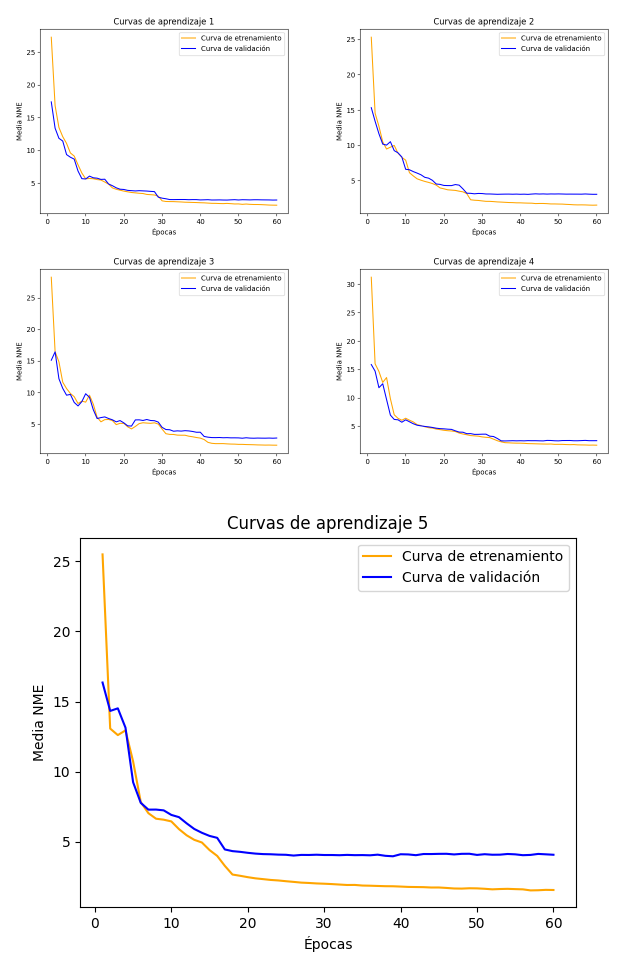
\includegraphics[width=0.9\textwidth]{img/curvas_aprendizaje_modelbase.png}
    \caption{Curvas de aprendizaje en cada partición del modelo base.}
    \label{fig:Curvas_modelbase}
\end{figure}

\newpage
\subsection*{Modelo de ajuste fino del encoder}
\begin{figure}[H]
    \centering
    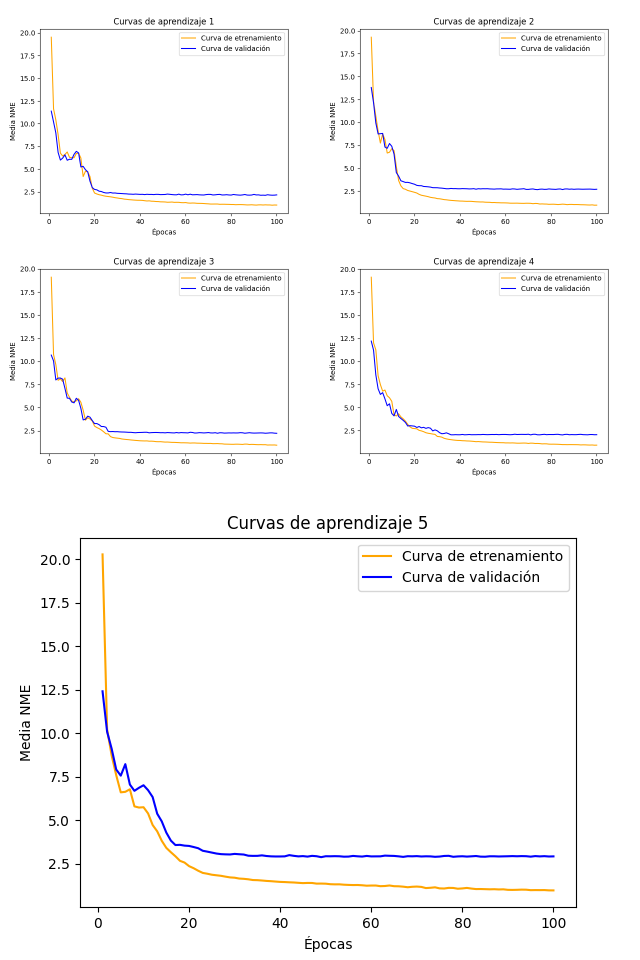
\includegraphics[width=0.9\textwidth]{img/curvas_encoder.png}
    \caption{Curvas de aprendizaje en cada partición del modelo de finetuning del encoder.}
    \label{fig:curvas_encoder}
\end{figure}

\newpage
\subsection*{Modelo de ajuste fino del decoder}
\begin{figure}[H]
    \centering
    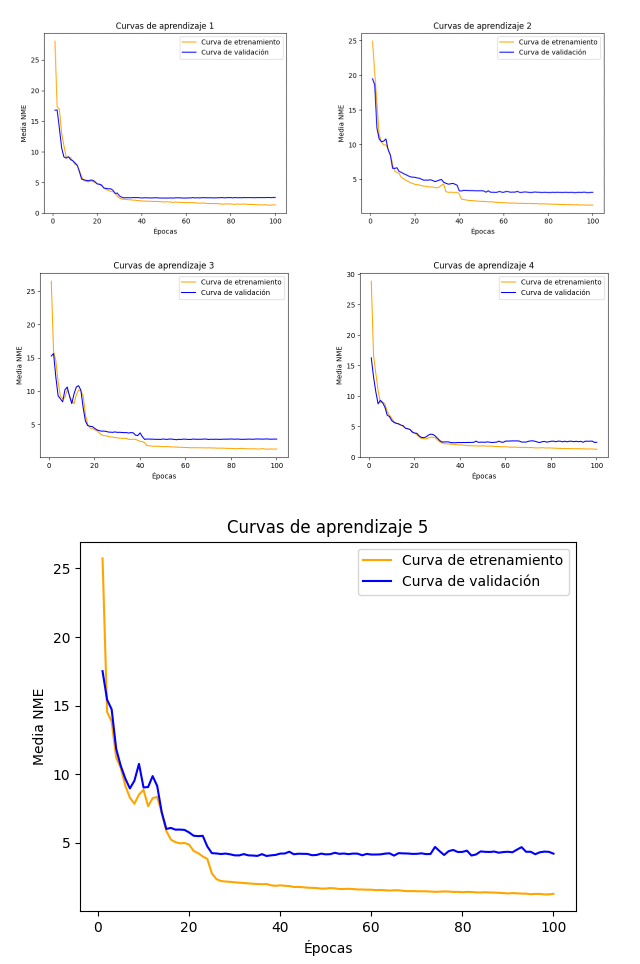
\includegraphics[width=0.9\textwidth]{img/curvas_decoder.png}
    \caption{Curvas de aprendizaje en cada partición del modelo de finetuning del encoder.}
    \label{fig:curvas_decoder}
\end{figure}

\newpage
\subsection*{Modelo con data augmentation}
\begin{figure}[H]
    \centering
    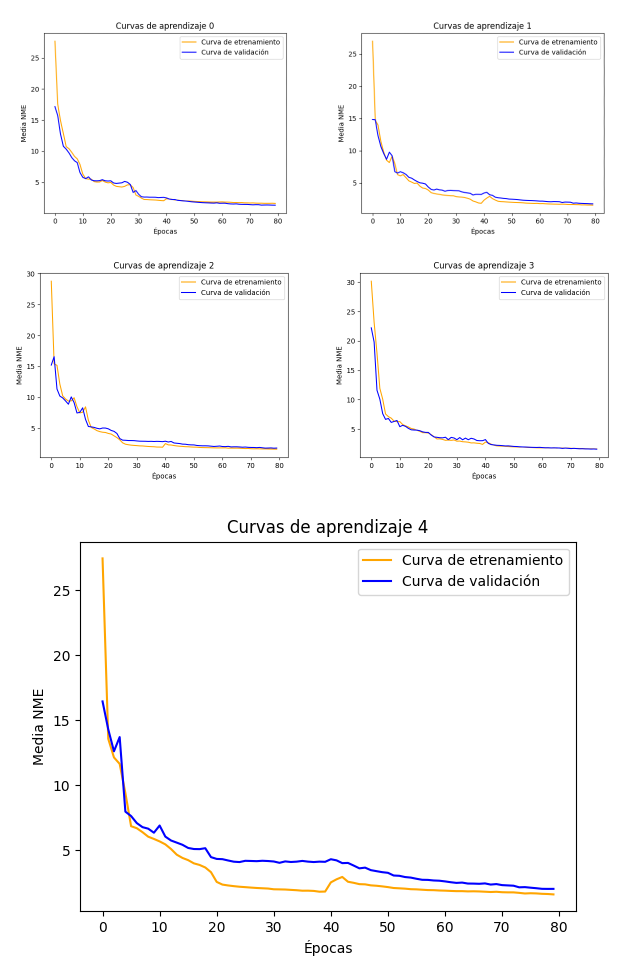
\includegraphics[width=0.9\textwidth]{img/curvas_daugmentation.png}
    \caption{Curvas de aprendizaje en cada partición del modelo de data augmentation.}
    \label{fig:curvas_daugmentation}
\end{figure}

\endinput
%------------------------------------------------------------------------------------
% FIN DEL APÉNDICE. 
%------------------------------------------------------------------------------------
